\section{Optik}
\subsection{Reflexionsgesetz}

\begin{center}
	\begin{minipage}{0.3\textwidth}
		\formula{$\varepsilon' = \varepsilon$} \\
	
		\unit{$\varepsilon$}{Einfalswinkel}{$rad$} \\
		\unit{$\varepsilon'$}{Ausfalswinkel}{$rad$}
	\end{minipage}%%% to prevent a space
	\begin{minipage}{0.3\textwidth}
		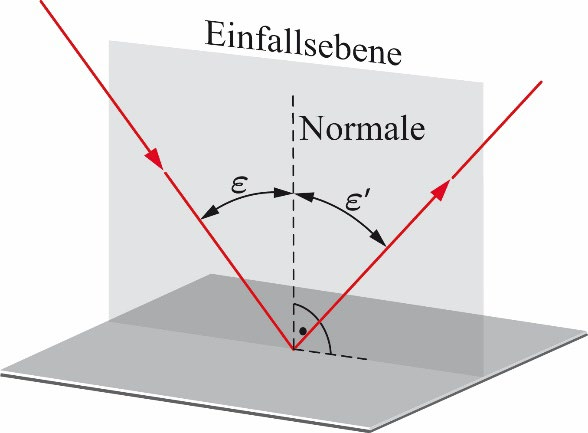
\includegraphics[height=2cm,keepaspectratio=true]{Images/reflexionsgesetz.png}
	\end{minipage}
\end{center}




\subsection{Brechungsgesetz}

Je nach Winkel und Material wird ein Teil reflektiert und ein Teil gebrochen. Ausserdem spielt die Polarisationsrichtung eine Rolle.
\begin{center}
	\begin{minipage}{0.3\textwidth}
		\formula{$\sin(\varepsilon_1) \cdot n_1 = \sin(\varepsilon_2) \cdot n_2 $} 
		\formula{$n = \dfrac{c}{u}$}\\
	
		\unit{$\varepsilon_1$}{Einfalswinkel}{$rad$} \\
		\unit{$\varepsilon_1'$}{Ausfalswinkel}{$rad$} \\
		\unit{$\varepsilon_2$}{Brechungswinkel}{$rad$} \\
		\unit{$n$}{Brechungsindex}{$1$} \\
		\unit{$c$}{Vakuum-Lichtgeschwindigkeit (299'792'458)}{$\frac{m}{s^2}$}	
	\end{minipage}%%% to prevent a space
	\begin{minipage}{0.3\textwidth}
		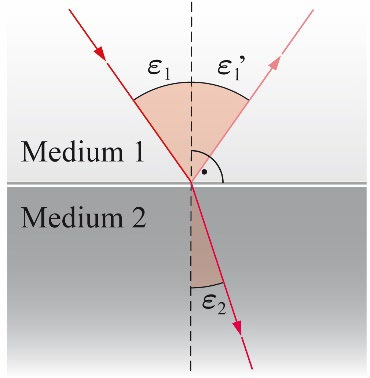
\includegraphics[height=2cm,keepaspectratio=true]{Images/brechungsgesetz.png}
	\end{minipage}
\end{center}




\subsection{Totalreflexion}

\begin{center}
	\begin{minipage}{0.1\textwidth}
		\formula{$\varepsilon_g = \arcsin(\frac{n_1}{n_2}) $}
	\end{minipage}%%% to prevent a space
	\begin{minipage}{0.5\textwidth}
		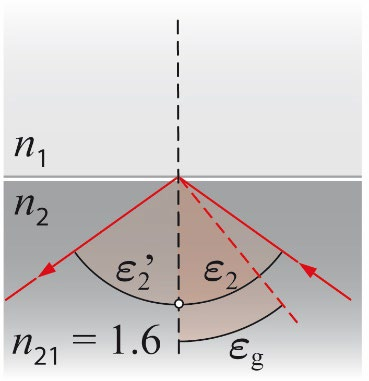
\includegraphics[height=2cm,keepaspectratio=true]{Images/totalreflexion.png}
		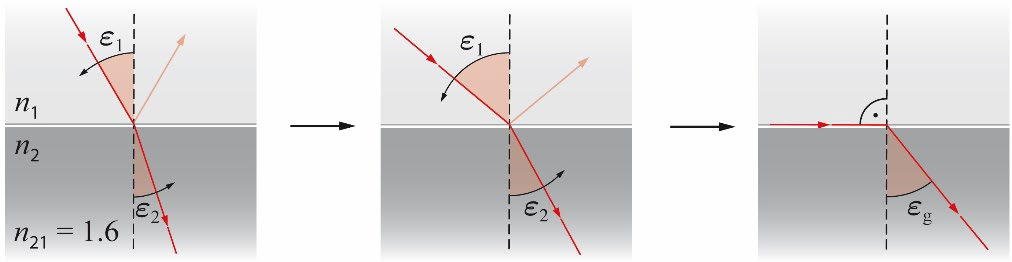
\includegraphics[height=2cm,keepaspectratio=true]{Images/einfalswinkel.png}
	\end{minipage}
\end{center}

\unit{$\varepsilon_g$}{Grenzwinkel}{$rad$} \\
\unit{$n_{1,2}$}{Brechungsindex}{$1$}




\subsection{Anwendungen}
\subsubsection{Prisma}

Die \textbf{Minimalablenkung} entsteht wenn der Einfallswinkel gleich dem Ausfallswinkel entspricht.

\begin{center}
	\begin{minipage}{0.3\textwidth}
		\formula{$ n_2 = n_1 \dfrac{\sin\left(\dfrac{\varphi}{2}\right)}{\dfrac{\delta_{min} + \varphi}{2}} $}
		\formula{$ \delta_{min} = 2 \arcsin(\frac{n_1}{n_2} \sin(\frac{\varphi}{2})) - \varphi $}
	
		Falls $ n_2 = 1 $ (Vakuum):
		\formula{$ n_1 = \dfrac{\sin\left(\frac{\varphi + \delta}{2}\right)}{\frac{\varphi}{2}} $}
	\end{minipage}%%% to prevent a space
	\begin{minipage}{0.3\textwidth}
		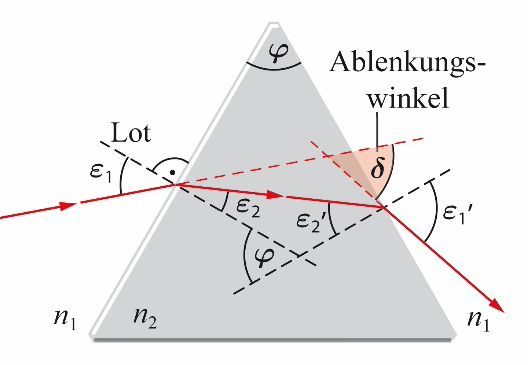
\includegraphics[height=3cm,keepaspectratio=true]{Images/prisma.png}
	\end{minipage}
\end{center}

\unit{$ n_1 $}{Brechungsindex Prisma}{$1$} \\
\unit{$ n_2 $}{Brechungsindex Medium}{$1$} \\
\unit{$ \varphi $}{Scheitelwinkel}{$rad$} \\
\unit{$ \delta $}{Ablenkwinkel}{$rad$} \\

\subsubsection{Lichtwellenleiter}

\begin{center}
	\begin{minipage}{0.3\textwidth}
		Falls $ n_1 > n2 $ :
		\formula{$ \alpha_{1max} = \arcsin\left( \dfrac{n_1 \cos(\arcsin(\frac{n_2}{n_1}))}{n_0} \right)  $}
		\formula{$ n_0 \sin(\alpha_1) = n_1 \sqrt{1 - \cos^2(\alpha_2)} $}
		\formula{$ n_0 \sin(\alpha_1) = n_1 \sqrt{1 - \left( \frac{n_2}{n_1} \right)^2 } $}
		\formula{$ n_0 \sin(\alpha_1) = \sqrt{n_1 ^2 - n_2 ^2} $}
	\end{minipage}%%% to prevent a space
	\begin{minipage}{0.3\textwidth}
		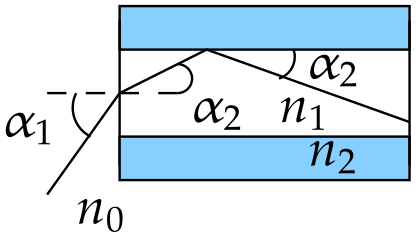
\includegraphics[height=3cm,keepaspectratio=true]{Images/lichtwellenleiter.png}
	\end{minipage}
\end{center}



\subsection{Dispersion}

\begin{center}
	\begin{minipage}{0.25\textwidth}
		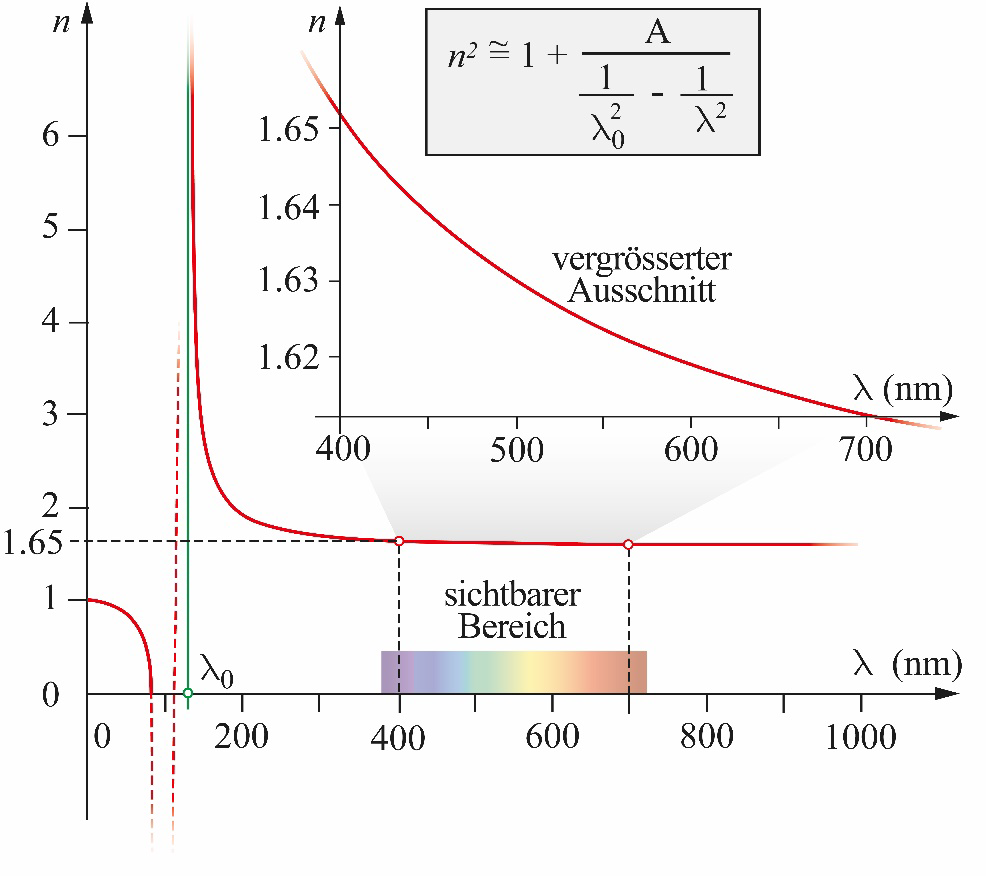
\includegraphics[height=5cm,keepaspectratio=true]{Images/dispersion_graph.png}
	\end{minipage}%%% to prevent a space
	\begin{minipage}{0.3\textwidth}
		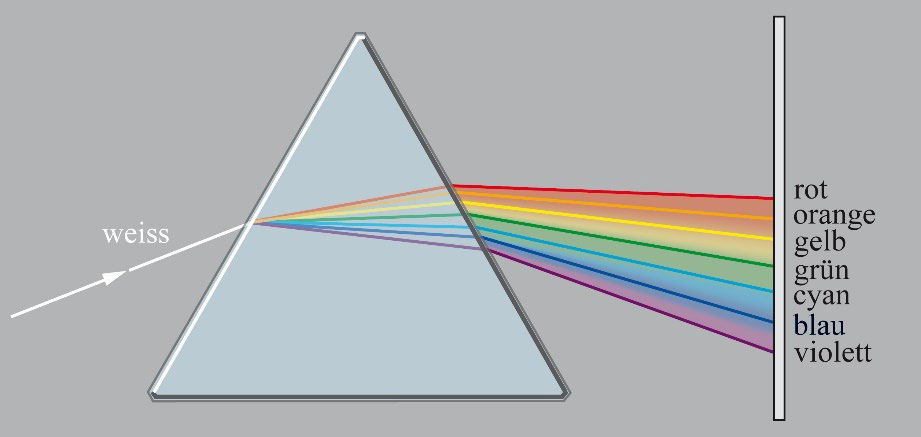
\includegraphics[height=3cm,keepaspectratio=true]{Images/dispersion_prisma.png}
	\end{minipage}
\end{center}


\subsection{Abbildungen}
\subsubsection{Allgemein}
\formula{$ \dfrac{b}{g} = \dfrac{B}{G} = \beta = \dfrac{b - f}{f} $}
\formula{$ \dfrac{1}{f} = \dfrac{1}{g} + \dfrac{1}{b}$} \\
\begin{center}
	\begin{minipage}{0.3\textwidth}
		\unit{$ b $}{Bildweite}{$ m $} \\
		\unit{$ g $}{Gegenstandsweite}{$ m $} \\
		\unit{$ B $}{Bildgrösse}{$ m $}
	\end{minipage}%%% to prevent a space
	\begin{minipage}{0.3\textwidth}
		\unit{$ G $}{Gegenstansgrösse}{$ m $} \\
		\unit{$ \beta $}{Abbildungsverhälltniss}{$ 1 $} \\
		\unit{$ f $}{Brennweite}{$ m $}
	\end{minipage}
\end{center}

\subsubsection{Spiegel}

\textbf{Planspiegel}
\begin{center}
	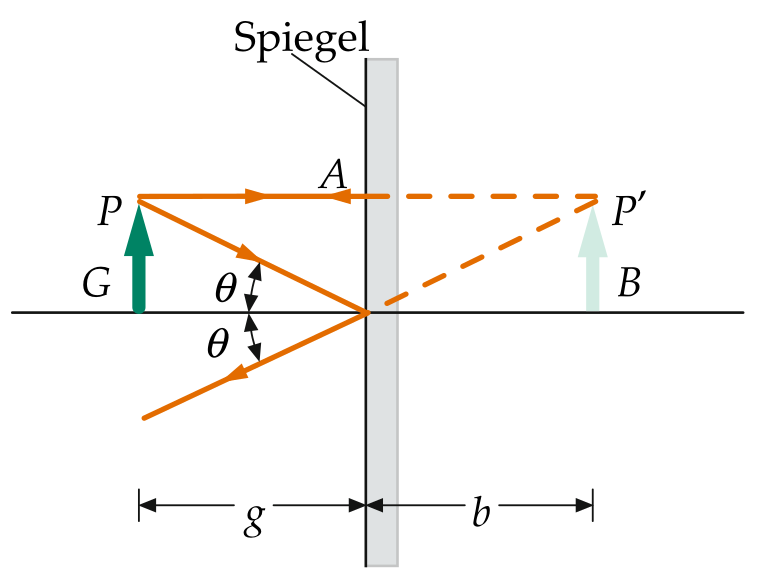
\includegraphics[height=3cm,keepaspectratio=true]{Images/planspiegel.png}
\end{center}


\textbf{Konkavspiegel}

\begin{center}
	\begin{minipage}{0.3\textwidth}
		Für Sphärische Spiegel gillt:
		\formula{$ f = \dfrac{r}{2} $}
	\end{minipage}%%% to prevent a space
	\begin{minipage}{0.3\textwidth}
		\unit{f}{Brennweite}{$m$} \\
		\unit{r}{Spiegelradius}{$m$}
	\end{minipage}
\end{center}

\begin{center}
	\begin{minipage}{0.3\textwidth}
		Gegenstand vor dem Brennpunkt. \\
		Erzeugt reeles Bild. \\
		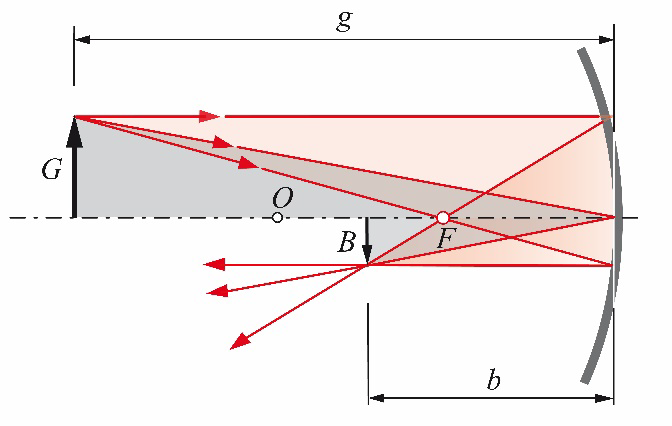
\includegraphics[height=3cm,keepaspectratio=true]{Images/konkavspiegel1.png}
	\end{minipage}%%% to prevent a space
	\begin{minipage}{0.3\textwidth}
		Gegenstand hinter dem Brennpunkt. \\
		Erzeugt virtuelles Bild. \\
		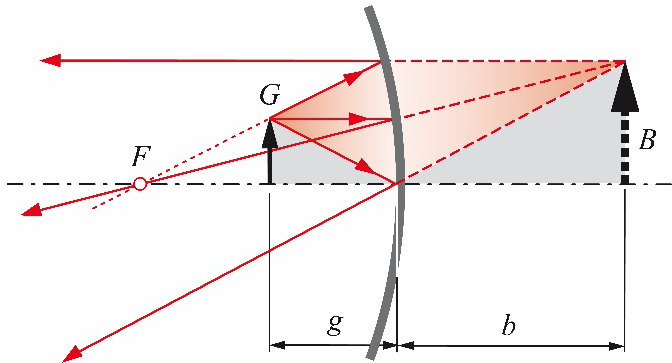
\includegraphics[height=3cm,keepaspectratio=true]{Images/konkavspiegel2.png}
	\end{minipage}
\end{center}


\textbf{Konvexspiegel}
\begin{center}
	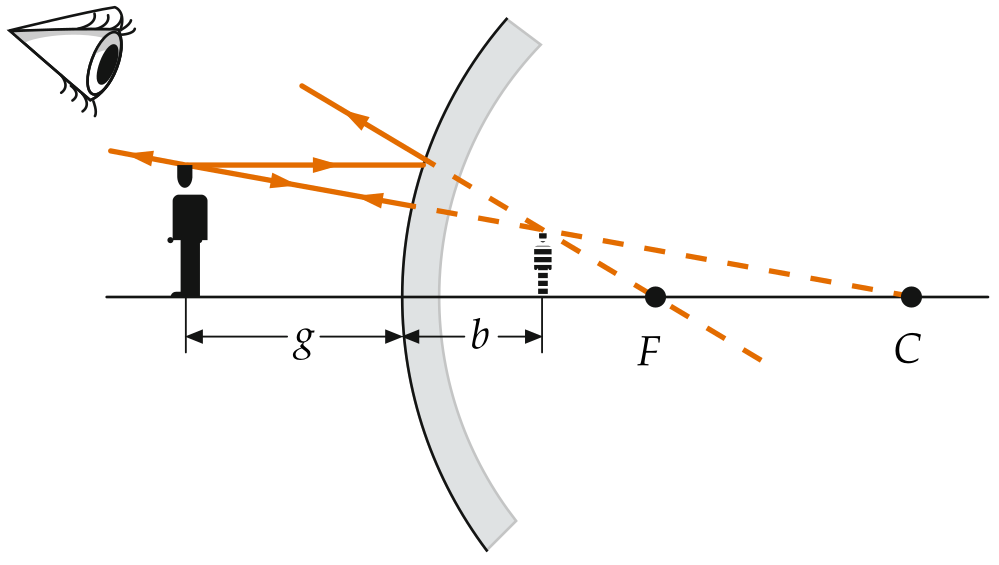
\includegraphics[height=3cm,keepaspectratio=true]{Images/konvexspiegel.png}
\end{center}

\subsubsection{Linsen}

\begin{center}
	\begin{minipage}{0.2\textwidth}
		\formula{$ D = \dfrac{1}{f} $}
		\formula{$ D = \left( \frac{n_2}{n_1} - 1 \right) \left( \frac{1}{r_1} + \frac{1}{r2} \right)  $} \\
		
		\unit{$ D $}{Brechkraft / Dioptrie}{$1$} \\
		\unit{$ f $}{Brennweite}{$m$} \\
		\unit{$ n_{1,2} $}{Brechungsindexe}{$1$} \\
		\unit{$ r_{1,2} $}{Radien von Linse}{$m$} \\
	\end{minipage}%%% to prevent a space
	\begin{minipage}{0.4\textwidth}
		\begin{itemize}
			\setlength\itemsep{-0.5 em}
			\item Für sammelde optische Bauelemente ist f > 0.
			\item Für zerstreuende optische Bauelemente f < 0.
			\item Für virtuelle Bilder ist b < 0 und B < 0.
			\item Für vortuelle Gegenstände ist g <	0 und G < 0.
		\end{itemize}
	\end{minipage}
\end{center}

\begin{center}
	\begin{minipage}{0.3\textwidth}
		Bündelnde Linse \\
		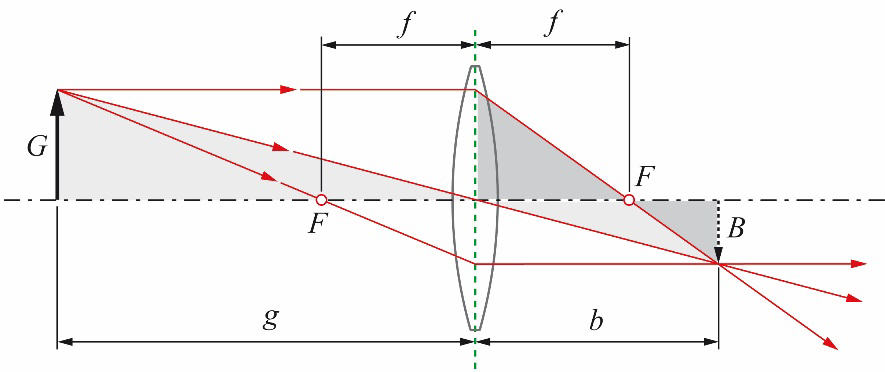
\includegraphics[height=3cm,keepaspectratio=true]{Images/buendelndelinse.png}
	\end{minipage}%%% to prevent a space
	\begin{minipage}{0.3\textwidth}
		Zerstreuende Linse \\
		Brechungsindex negativ! \\
		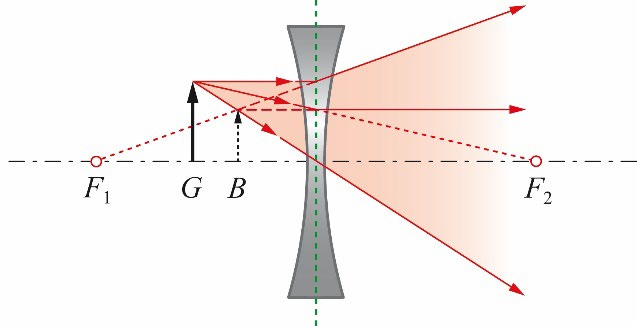
\includegraphics[height=3cm,keepaspectratio=true]{Images/streuendelinse.png}
	\end{minipage}
\end{center}

\subsection{Abbildungssysteme}

\unit{$ \varepsilon $}{Sehwinkel}{Bogenminute | arcmin | $ 1^\circ = 60\SIUnitSymbolArcminute $} \\
\unit{$ s $}{deutliche Sehweite (normiert = 25cm)}{m}



\subsubsection{Auflösung, Sehwinkel und Sehweite}

\textbf{Auflösung}: Minimaler Winkelabstand $\varepsilon_min$ zwischen zweier Punkte, welche noch
unterschieden werden können.
\textbf{Sehweite}: Distanz, in der ein Gegenstand noch scharf gesehen werden kann.

Die menschliche Sehschärfe beträgt ca. 1\SIUnitSymbolArcminute.

\begin{center}
	\begin{minipage}{0.2\textwidth}
		\formula{$ S = \dfrac{1}{\varepsilon_{min}} $} \\
		\unit{$S$}{Sehschärfe}{$\frac{1}{arcmin}$} \\
		\unit{$\varepsilon$}{Sehwinkel}{$arcmin$} \\
	\end{minipage}%%% to prevent a space
	\begin{minipage}{0.3\textwidth}
		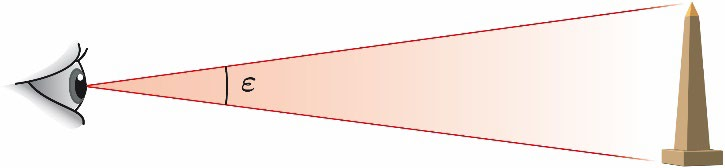
\includegraphics[height=2cm,keepaspectratio=true]{Images/sehwinkel.png}
	\end{minipage}
\end{center}




\subsubsection{Kamera}

\begin{center}
	\begin{minipage}{0.26\textwidth}
		\formula{$ H = \left( \dfrac{d}{f} \right)^2 = q^2 $}
		\formula{$ \dfrac{1}{g} = \dfrac{1}{g_0} \pm \dfrac{u}{q \cdot f^2} $}
		\formula{$ I \sim d^2 $}
		\formula{$ B = \dfrac{f}{g - f} \cdot G $}
		\formula{$ Z = \dfrac{1}{q} = \dfrac{d}{f} $}
		\formula{$ H \sim \dfrac{I}{B^2} \sim \dfrac{d^2}{f^2} $}
	\end{minipage}%%% to prevent a space
	\begin{minipage}{0.3\textwidth}
		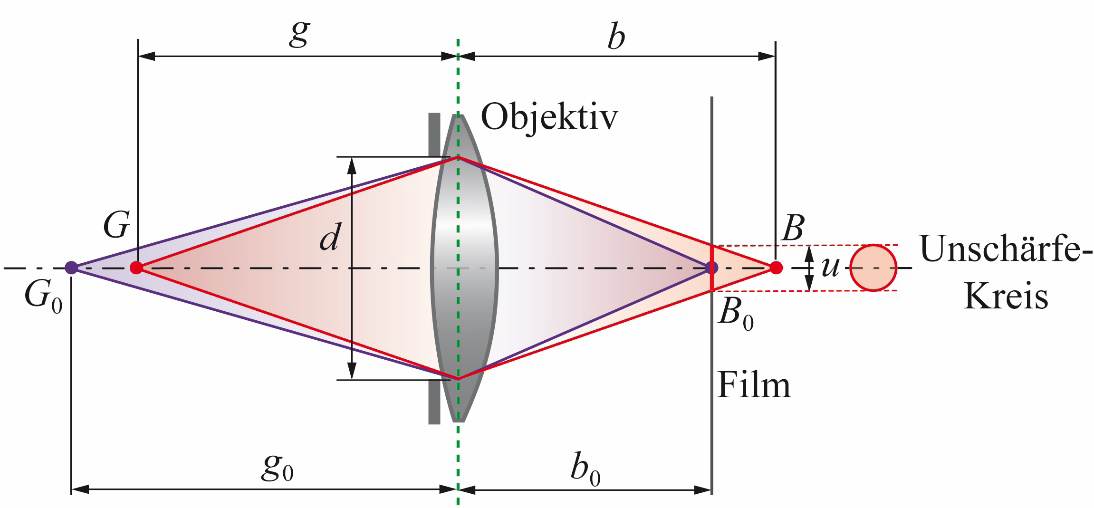
\includegraphics[height=3cm,keepaspectratio=true]{Images/kamera.png}
	\end{minipage}
\end{center}

\begin{center}
	\begin{minipage}{0.3\textwidth}
		\unit{$ B $}{Bildgrösse}{$ m $} \\
		\unit{$ G $}{Gegenstandsgrösse}{$ m $} \\
		\unit{$ H $}{Lichtstärke (Helligkeit)}{$ \frac{W}{m^2} $} \\
		\unit{$ I $}{Lichtstrom}{$ W $} \\
		\unit{$ Z $}{Öffnungsverhältnis}{$ 1 $} \\
		\unit{$ b $}{Bildweite}{$ m $} \\
		\unit{$ b_0 $}{Filmweite}{$ m $} \\
	\end{minipage}%%% to prevent a space
	\begin{minipage}{0.3\textwidth}
		\unit{$ d $}{Durchmesser Eintrittspupille}{$ m $} \\
		\unit{$ f $}{Brennweite}{$ m $} \\
		\unit{$ g $}{Gegenstandsweite}{$ m $} \\
		\unit{$ g_0 $}{Schärfentiefenbereich}{$ m $} \\
		\unit{$ q $}{Blendenzahl}{$ \frac{\sqrt{W}}{m} $} \\
		\unit{$ u $}{Unschärfenkreis-Durchmesser}{$ m $} \\
	\end{minipage}
\end{center}




\subsubsection{Lupe}

\begin{center}
	\begin{minipage}{0.18\textwidth}
		\formula{$ V = \dfrac{\tan(\varepsilon)}{\tan(\varepsilon_0)} = \dfrac{s}{f} $}
		\formula{$ \tan(\varepsilon) = \dfrac{G}{f} $}
		\formula{$ \tan(\varepsilon_0) = \dfrac{G}{s} $}\\
		
		\unit{$ V $}{Vergrösserung}{$1$} \\
		\unit{$ G $}{Gegenstandsgrösse}{$m$} \\
		\unit{$ \varepsilon $}{Sehwinkel}{$rad$} \\
		\unit{$ \varepsilon_0 $}{Sehwinkel ohne Lupe}{$rad$} \\
		\unit{$ s $}{deutliche Sehweite}{$m$} \\
		\unit{$ f $}{Brennweite}{$m$} \\
	\end{minipage}%%% to prevent a space
	\begin{minipage}{0.3\textwidth}
		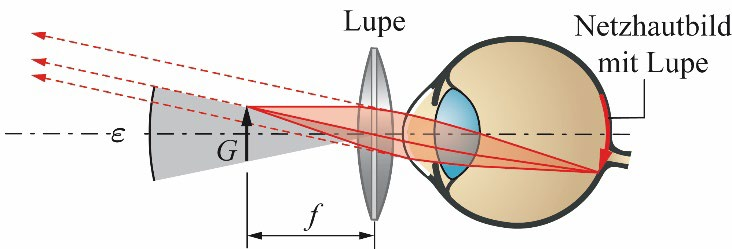
\includegraphics[height=2cm,keepaspectratio=true]{Images/lupe.png}
		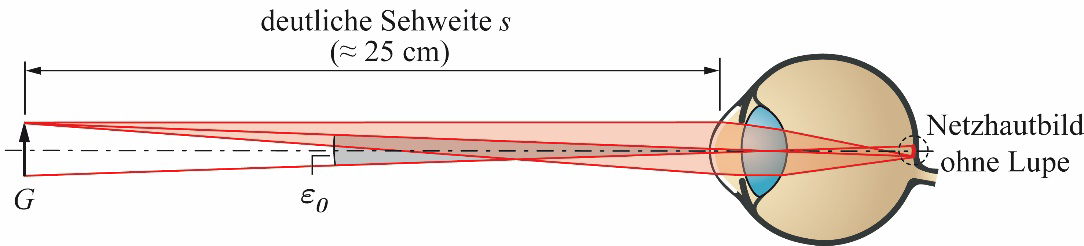
\includegraphics[height=2cm,keepaspectratio=true]{Images/deutliche_sichtweite.png}
	\end{minipage}
\end{center}





\subsubsection{Mikroskop}

\begin{center}
	\begin{minipage}{0.18\textwidth}
		\formula{$ V = \dfrac{\tan(\varepsilon)}{\tan(\varepsilon_0)} $}
		\formula{$ V = \dfrac{\Delta}{f_1} \dfrac{s}{f_2} $}
		\formula{$ V = \dfrac{B}{G} \dfrac{s}{f_2} = \dfrac{b_1}{g_1} \dfrac{s}{f_2} $}
	\end{minipage}%%% to prevent a space
	\begin{minipage}{0.3\textwidth}
		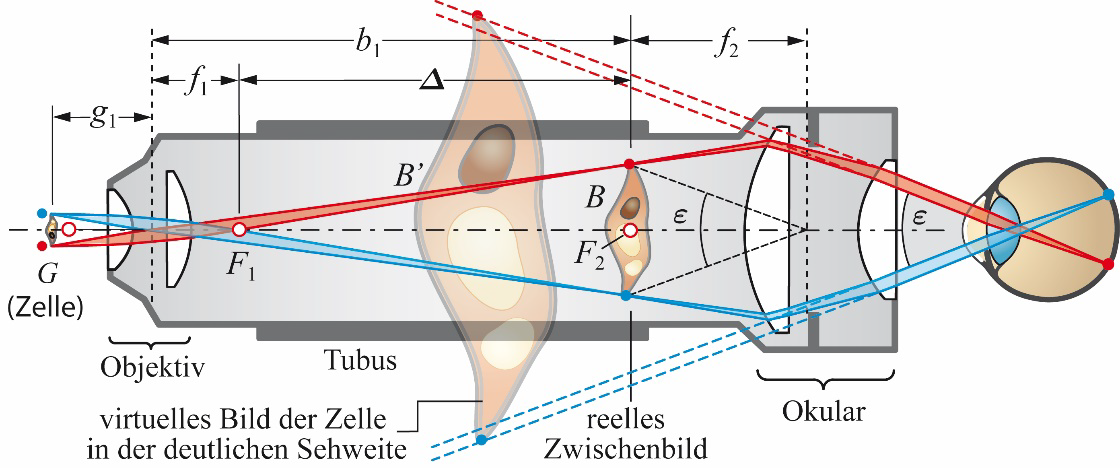
\includegraphics[height=3.5cm,keepaspectratio=true]{Images/mikroskop.png}
	\end{minipage}
\end{center}

\begin{center}
	\begin{minipage}{0.3\textwidth}
		\unit{$ B $}{Bildgrösse}{$m$} \\
		\unit{$ G $}{Gegenstandsgrösse}{$m$} \\
		\unit{$ V $}{Vergrösserung}{$1$} \\
		\unit{$ \varepsilon $}{Sehwinkel}{$rad$} \\
		\unit{$ \varepsilon_0 $}{Sehwinkel ohne Mikroskop}{$rad$} \\
	\end{minipage}%%% to prevent a space
	\begin{minipage}{0.3\textwidth}
		\unit{$ b_1 $}{Bildweite}{$m$} \\
		\unit{$ f_1 $}{Brennweite Objektiv}{$m$} \\
		\unit{$ f_2 $}{Brennweite Okular}{$m$} \\
		\unit{$ s $}{deutliche Sehweite}{$m$} \\
		\unit{$ \Delta $}{Tubuslänge}{$m$} \\
	\end{minipage}
\end{center}


\subsubsection{Vernrohr}

\begin{center}
	\begin{minipage}{0.2\textwidth}
		\formula{$ V = \dfrac{\tan(\varepsilon)}{\tan(\varepsilon')} = \dfrac{f_1}{f_2}$}
	\end{minipage}%%% to prevent a space
	\begin{minipage}{0.3\textwidth}
		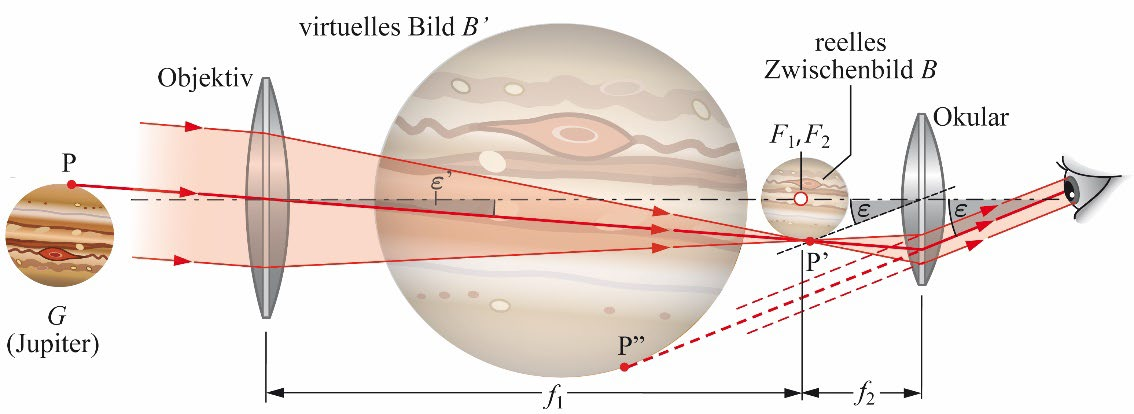
\includegraphics[height=3cm,keepaspectratio=true]{Images/vernrohr.png}
	\end{minipage}
\end{center}

\begin{center}
	\begin{minipage}{0.3\textwidth}
		\unit{$ V $}{Vergrösserung total}{$1$} \\
		\unit{$ f_1 $}{Brennweite Objektiv}{$m$} \\
		\unit{$ f_2 $}{Brennweite Okular}{$m$} \\
	\end{minipage}%%% to prevent a space
	\begin{minipage}{0.3\textwidth}
		\unit{$ \varepsilon $}{Ausfallswinkel}{$rad$} \\
		\unit{$ \varepsilon' $}{Einfallswinkel}{$rad$} \\
	\end{minipage}
\end{center}

\subsection{Farbenlehre}

\begin{center}
	\begin{minipage}{0.2\textwidth}
		Subtraktiv \\
		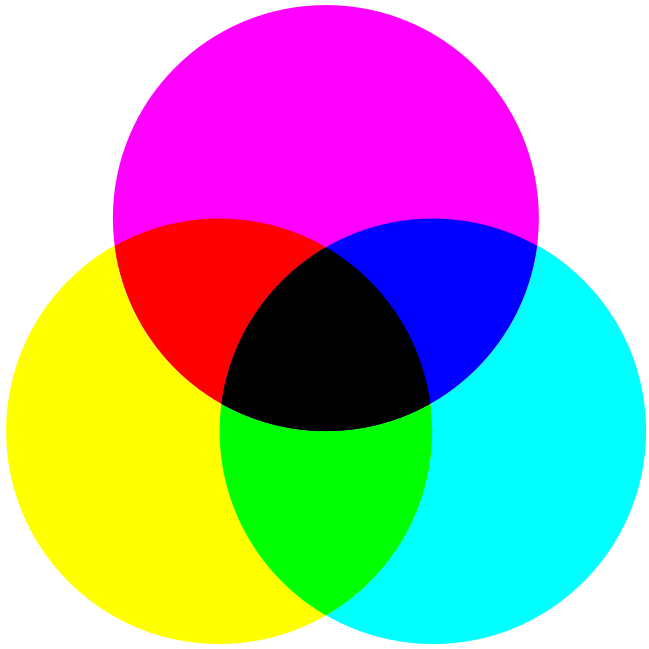
\includegraphics[height=2cm,keepaspectratio=true]{Images/farbenkreise_subtraktiv.png}
	\end{minipage}%%% to prevent a space
	\begin{minipage}{0.2\textwidth}
		Additiv \\
		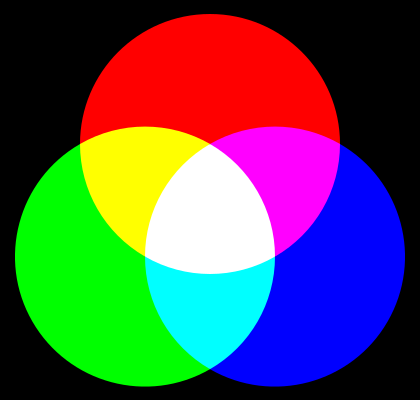
\includegraphics[height=2cm,keepaspectratio=true]{Images/farbenkreise_additiv.png}
	\end{minipage}
\end{center}
